\documentclass[11pt,a4paper]{article}
\usepackage[margin=2.1cm]{geometry}
\usepackage[T1]{fontenc}
\usepackage{mathptmx}\usepackage[scaled=0.92]{helvet}
\usepackage{microtype}
\usepackage{graphicx}
\usepackage{booktabs}
\usepackage{tabularx}
\usepackage{xcolor}
\usepackage{amsmath}
\usepackage{enumitem}
\usepackage{caption}
\usepackage{xurl}\usepackage[hidelinks]{hyperref}
\usepackage{fancyhdr}
\usepackage{float}

\graphicspath{{../results/figures/}}
\captionsetup{font=small,labelfont=bf,skip=4pt}
\setlist{itemsep=1pt,topsep=3pt,leftmargin=*}
\setlength{\parskip}{3pt}
\setlength{\parindent}{0pt}
\newcommand{\todo}[1]{\colorbox{yellow}{\textbf{TO FILL:} #1}}
\pagestyle{fancy}\fancyhf{}\renewcommand{\headrulewidth}{0pt}
\fancyfoot[C]{\small\thepage}\fancyfoot[R]{\small BT4012 Group 20}

\begin{document}

\begin{center}
{\LARGE\bfseries Who Should Medicare Audit Next?}\\[3pt]
{\large Provider Fraud Ranking Beyond Provider Size, with an Agent-Assisted Investigation Layer}\\[8pt]
BT4012 Fraud Analytics, Group 20\\
\todo{member names and student numbers}\\[3pt]
Code and reproduction instructions: \todo{GitHub URL}
\end{center}

\noindent\textbf{Summary.} We rank 5,410 Medicare providers for audit from 558,211 claims. The key finding is that the PotentialFraud label is largely a size signal: ranking providers by total reimbursement alone, with no model, gives a cross-validated PR-AUC of 0.674 and ROC-AUC of 0.934, close to the 0.95 ROC-AUC that published models report on this dataset. Our best model (LightGBM) adds a consistent but modest margin (PR-AUC 0.732, better on 25 of 25 folds; 0.805 vs 0.743 on the held-out test set). A model given no size features still reaches 0.714, and the size-free signal sits almost entirely in care intensity: length of stay and claims per patient. Network features, resampling and expert rules add nothing. We also show that a claim-level random split, common in public work on this dataset, inflates claim-level PR-AUC from 0.542 to 0.868 because 93.6\% of physicians bill for a single provider. The LLM agents did not improve the model (0.716 averaged over three runs) because the Critic applied an unpaired significance rule, but the Leakage agent caught 15 of 15 planted leaks and the retrieval-grounded case briefs were fully faithful and downgraded size-only cases from audit to desk review.

%=====================================================================
\section{Problem description}

\textbf{The fraud problem.} Medicare pays providers (hospitals, clinics, practices) for care billed through claims. Provider fraud takes the form of billing for services not provided, duplicate claims, misrepresented services, upcoding to more expensive services, and billing non-covered services as covered \cite{kaggle}. It is a provider-level behaviour: one claim rarely looks abnormal, but a provider's billing pattern can. Payers respond by auditing providers, and audit capacity is small relative to the number of providers.

\textbf{Our question.} Given a fixed audit capacity, which providers should be audited first, and what evidence supports each flag? We treat this as a \emph{ranking} problem evaluated on the top of the queue, not as accuracy on all providers. Midway through the project the data reframed the question (Section~\ref{sec:data}): because provider size alone explains most of the label, we ask \emph{what a model finds that size alone does not}.

\textbf{Who is affected and why it is hard.} Payers and taxpayers bear the losses; honest providers bear the cost of false accusations and audits. Detection is hard for four reasons that lectures 01 and 03 name: (i) fraud is rare, 9.35\% of providers here, so accuracy is misleading; (ii) fraudsters blend in, so single claims look normal; (iii) labels are uncertain, and here their origin is undocumented; (iv) large legitimate providers bill more of everything, so a model can confuse size with suspicion and penalise big hospitals.

\textbf{Contributions.} (1) A size-alone baseline (E0) that every model must beat, and a size-free model that shows what remains; (2) a leakage-safe evaluation with 25 repeated folds, a once-opened test set and bootstrap intervals, plus a demonstration of how much a leaky split inflates results (E9); (3) an agent layer whose decisions are structured, executed by code and measured against a fixed pipeline, with retrieval-grounded case briefs for investigators.

%=====================================================================
\section{Data overview}\label{sec:data}

\textbf{Source.} The Kaggle \emph{Healthcare Provider Fraud Detection Analysis} dataset \cite{kaggle}: four labelled training files (provider labels, beneficiaries, inpatient and outpatient claims) and four unlabelled test files. Kaggle's test files carry no labels, so all evaluation uses the 5,410 labelled providers; the unlabelled files are not used.

\textbf{Label provenance and validity.} The dataset page does not say how \texttt{PotentialFraud} was assigned. The claims match the layout of CMS's synthetic 2008--2010 DE-SynPUF files (ten diagnosis and six procedure codes, chronic-condition flags coded 1/2, renal disease coded 0/Y, a 2008--2009 window) \cite{synpuf}. CMS states that DE-SynPUF payments were coarsened, dates perturbed and provider codes randomised, and warns that provider-level inference from it is misleading \cite{synpufdug}. Consistent with this, 99.2\% of inpatient payments are exact multiples of \$1,000. We therefore treat the label as ``previously flagged as potentially fraudulent'' and frame every conclusion as a statement about this benchmark, not about real providers. This answers the lecturer's question on what our results can support.

\begin{table}[H]\centering\small
\caption{Dataset characteristics (training files).}\label{tab:data}
\begin{tabularx}{\linewidth}{lX}
\toprule
Providers & 5,410 labelled: 506 flagged, 4,904 not (9.35\%) \\
Claims & 558,211: 40,474 inpatient, 517,737 outpatient; 138,556 beneficiaries \\
Time range & 27 Nov 2008 to 31 Dec 2009 (inpatient from 27 Nov 2008, outpatient from 12 Dec 2008) \\
Variables & Claims: 30 inpatient / 27 outpatient columns (IDs, dates, reimbursement, deductible, 3 physician IDs, admit and 10 diagnosis codes, 6 procedure codes, DRG). Beneficiaries: 25 columns (DOB, DOD, gender, race, state, county, renal disease, 11 chronic conditions, coverage months, annual reimbursement and deductibles) \\
Integrity checks & 0 duplicate claim IDs, 0 claims ending before they start, 0 discharges before admission, 0 claims after death, 0 claims from unlabelled providers \\
\bottomrule
\end{tabularx}
\end{table}

\begin{figure}[H]\centering
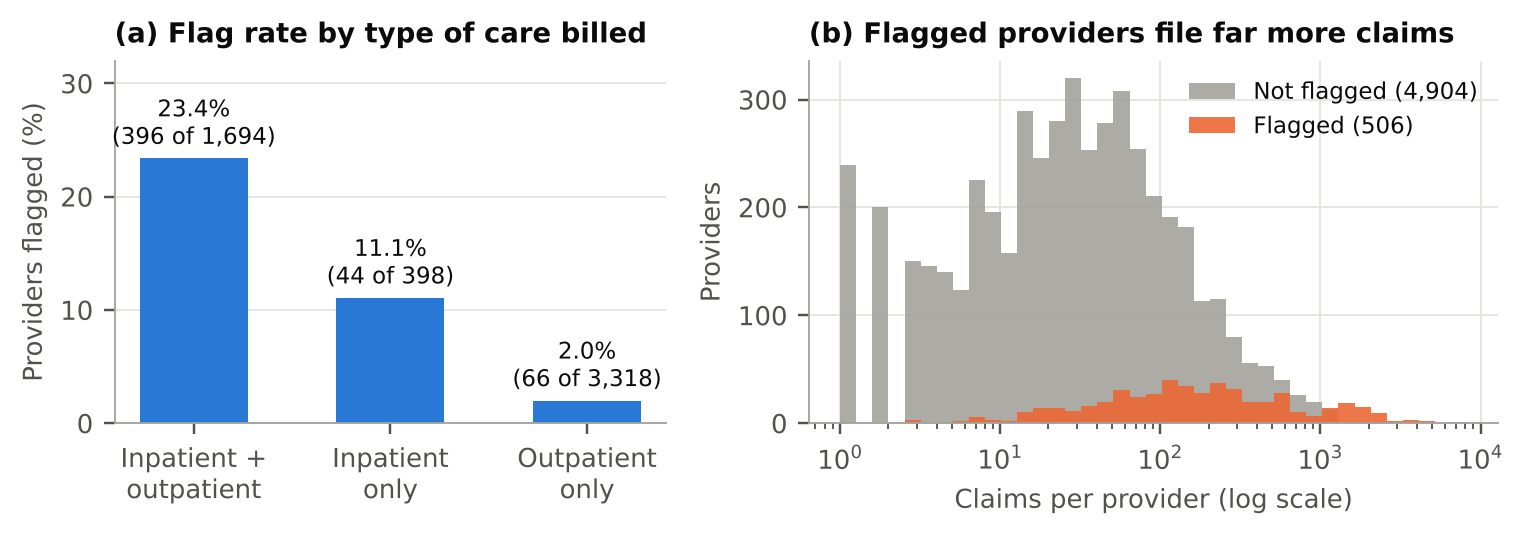
\includegraphics[width=\linewidth]{fig1_data.png}
\caption{(a) Providers billing inpatient care are flagged 5--12 times as often as outpatient-only providers, who are 61\% of all providers. (b) Flagged providers file a median of 155.5 claims against 27; they file 38.1\% of all claims and receive 53.1\% of all reimbursement.}\label{fig:data}
\end{figure}

\textbf{What the exploration showed.} Three facts shape the method. First, \emph{size dominates}: the 50 providers with the most claims are all flagged. Second, \emph{type of care matters}: billing inpatient care is itself a strong signal (Fig.~\ref{fig:data}a), so results are reported overall and the feature set encodes service mix. Third, \emph{missingness is structural}: operating physician is blank on 41.1\% of inpatient claims and procedure codes on 99.97\% of outpatient claims because many encounters involve no surgery, so values are counted, never imputed. Amounts are coarsened, so Benford's law, which assumes unconstrained values spanning orders of magnitude (lecture 02), is not applicable and we do not use it. Two-thirds (66.1\%) of beneficiaries see more than one provider, which gives a dense provider network for lecture 08 methods.

%=====================================================================
\section{Methodology}

\subsection{Preprocessing and feature engineering}

\textbf{Cleaning.} Chronic-condition flags and gender are recoded from 1/2 to 1/0 and renal disease from 0/Y to 0/1. The inpatient deductible equals \$1,068 on every non-blank claim, so it carries no information and is dropped. Dates are parsed to compute length of stay, claim duration and age at claim.

\textbf{Aggregation to providers.} The label is assigned per provider, so claims are aggregated to one row per provider. Aggregating also removes the claim-level leakage that Section~\ref{sec:e9} measures: a provider can appear in only one split. Table~\ref{tab:feat} lists the 63 features in eight families. The \emph{size} family holds raw counts and totals that grow with volume; every other family is a ratio, mean or share that describes \emph{how} a provider bills rather than \emph{how much}. This split is what lets us test what a model finds beyond size. Inpatient statistics are undefined for outpatient-only providers; they are set to 0 and the \texttt{has\_ip} flag tells models the zero is structural. Full definitions are in \texttt{src/fraudrank/features.py}.

\begin{table}[H]\centering\small
\caption{Provider features by family.}\label{tab:feat}
\begin{tabularx}{\linewidth}{lcX}
\toprule
Family & $n$ & Examples \\
\midrule
Size & 13 & claims, inpatient and outpatient claims, beneficiaries, total and inpatient reimbursement, distinct physicians, states, DRGs \\
Service mix & 4 & bills inpatient / outpatient care, inpatient share of claims and of reimbursement \\
Money & 9 & reimbursement per claim and per beneficiary, mean and max inpatient payment, outpatient deductible, share of zero payments \\
Intensity & 6 & mean and max length of stay, share of stays $\ge$10 days, claim duration, claims per beneficiary \\
Coding & 6 & diagnoses per claim, procedures per inpatient claim, surgery share, DRGs per inpatient claim, distinct primary diagnoses per claim \\
Physicians & 5 & claims per attending physician, top physician's share, attending = operating share \\
Duplication & 2 & share of claims matching another on patient, date, diagnosis and amount (same provider; any provider) \\
Patient mix & 18 & mean age, share deceased, chronic-condition count and 11 condition shares, renal share, patients' annual reimbursement \\
\bottomrule
\end{tabularx}
\end{table}

\subsection{Model selection and justification}

Models were chosen to answer specific questions, from no model to a flexible one (Table~\ref{tab:models}). Gradient boosting and SHAP are not covered in the lectures and are added for the reasons given.

\begin{table}[H]\centering\small
\caption{Models, why each is included, and its limitation here.}\label{tab:models}
\begin{tabularx}{\linewidth}{p{2.5cm}XX}
\toprule
Model & Why it fits this problem & Assumption / limitation \\
\midrule
Size alone (E0) & Ranks by one size measure, no fitting. Sets the bar any model must clear and tests whether the label is a volume signal. & Cannot separate a large honest hospital from a large suspicious one. \\
Expert rules & What a payer runs without ML (lecture 01): six red-flag measures, each firing above the training-fold 90th percentile; score = rules fired. & Hand-chosen thresholds; brittle; ties broken by reimbursement. \\
Logistic regression & Interpretable baseline (lecture 03) with calibrated probabilities, so P(flag) $\times$ amount gives an expected loss. L2 penalty, log1p + standardisation for skewed counts. & Linear in log-features; misses interactions such as ``inpatient and long stays''. \\
Random forest & Non-linear, robust to outliers and skew, little tuning. & Probabilities poorly calibrated; slow; less accurate than boosting on tabular data. \\
LightGBM \cite{lightgbm} & Gradient-boosted trees: handles skew, interactions and structural zeros natively; strong on small tabular data; per-provider explanations via exact TreeSHAP \cite{treeshap}. & Most tuning; opaque without SHAP; can overfit small folds. \\
Isolation Forest & Unsupervised anomaly detection (lecture 01): ignores the possibly noisy label. & Anomalous $\neq$ flagged: large honest providers are also anomalies. \\
Network features & Lecture 08: fraud is organised, so links through shared patients may carry signal. Personalised PageRank from flagged providers and neighbours' flag share. & Labels must be fold-local (below); large providers are linked to many others by chance. \\
\bottomrule
\end{tabularx}
\end{table}

A feedforward network or autoencoder (lecture 04) was not used: with 4,328 training providers and 63 tabular features, gradient boosting is the stronger and more interpretable choice, and the autoencoder's premise (fraud is reconstructed poorly) is already tested more directly by Isolation Forest.

\textbf{Network construction (lecture 08).} Providers are linked when they bill the same beneficiary, weighted by the number shared (5,410 nodes, 168,104 weighted links). Structure uses claims only, which are known for every provider at scoring time. Labels enter only through seeds: validation and test providers are scored with personalised PageRank seeded on training-fold flagged providers, and each training provider gets an out-of-fold value from five inner folds, so no provider sees its own label. We use the PageRank \emph{lift} (fraud-seeded score divided by the score seeded on all labelled providers) so that sheer connectivity does not masquerade as risk.

\textbf{Class imbalance.} Class weights are the default because they keep every real provider and add no synthetic ones. SMOTE \cite{smote} is tested as an alternative, applied inside each training fold only.

\subsection{Agent layer}\label{sec:agents}

Following the proposal, six LLM agents make decisions that code carries out. Each agent returns a schema-constrained JSON object (closed sets and bounded numbers), validated with pydantic and retried once on failure (lecture 05). Lecture 05 recommends temperature 0 for auditable output, but current Claude models no longer accept sampling parameters, so reproducibility comes from logging instead: every request and response is cached, and the agent experiments replay from that cache without an API key. Untrusted text is wrapped in tags declared to be evidence, not instructions.

\begin{itemize}
\item \textbf{Build time.} The \emph{Cleaning} agent proposes a cleaning plan that a team member approves; it is scored against a seven-item reference checklist from our profiling. The \emph{Feature} agent proposes provider features in a restricted grammar (an aggregation of an allowed claim column, or a ratio of allowed provider totals), which the executor computes. The \emph{Leakage} agent reviews every feature specification; it does not enforce the split, which code enforces. The \emph{Experiment} and \emph{Critic} agents run as one capped loop (at most three rounds) that sees cross-validation results on the first CV repeat only, never the test set.
\item \textbf{Run time.} For each provider at the top of the queue, the \emph{Case-file} agent receives structured evidence from code (the five largest SHAP drivers with values and peer percentiles among providers of the same care type) and unstructured evidence from a ten-section typology playbook we wrote (the five Kaggle schemes plus five provider patterns, each listing the features that can reveal it). Retrieval is hybrid (lecture 06): BM25 for exact terms and a dense latent-semantic index, fused by reciprocal rank \cite{rrf}, with one focused query per driver.
\end{itemize}

Each agent has its own test: E4 compares the agent pipeline with the fixed pipeline on identical folds over three independent runs, and with the Critic or the Feature agent removed; E8 checks every case brief deterministically (numbers copied correctly, cited section exists and lists one of the brief's drivers, no claim that fraud is confirmed); E10 plants five leaks among ten clean features and counts what the Leakage agent catches.

%=====================================================================
\section{Experiments and results}

\textbf{Protocol.} A stratified 80/20 provider split gives a development set (4,328 providers) and a test set (1,082 providers, 101 flagged) that was scored once, after all choices were fixed. Model selection uses $5\times5$ repeated stratified cross-validation on the development set (25 folds); results are mean $\pm$ SD over folds, and paired comparisons use the same folds. Hyperparameters were tuned on small grids scored on the first repeat only (LightGBM: 31 leaves, learning rate 0.02, 400 trees, colsample 0.5; random forest: min leaf 10, 30\% features; logistic: $C=0.3$). A time-based split is not possible: the label is a single flag per provider for the whole 13-month window.

\textbf{Metrics.} PR-AUC is primary because positives are rare and ROC-AUC rewards ordering the many negatives no investigator sees \cite{saito}. Precision@$k$ and recall@$k$ describe an audit queue of size $k$. Following the lecturer's feedback, $k$ is matched to the test set: 50 and 100 (best achievable precision 1.0) and 5\% and 10\% of providers. Test results carry stratified bootstrap 95\% intervals (2,000 resamples).

\subsection{E0--E1: models against size alone}

\begin{figure}[H]\centering
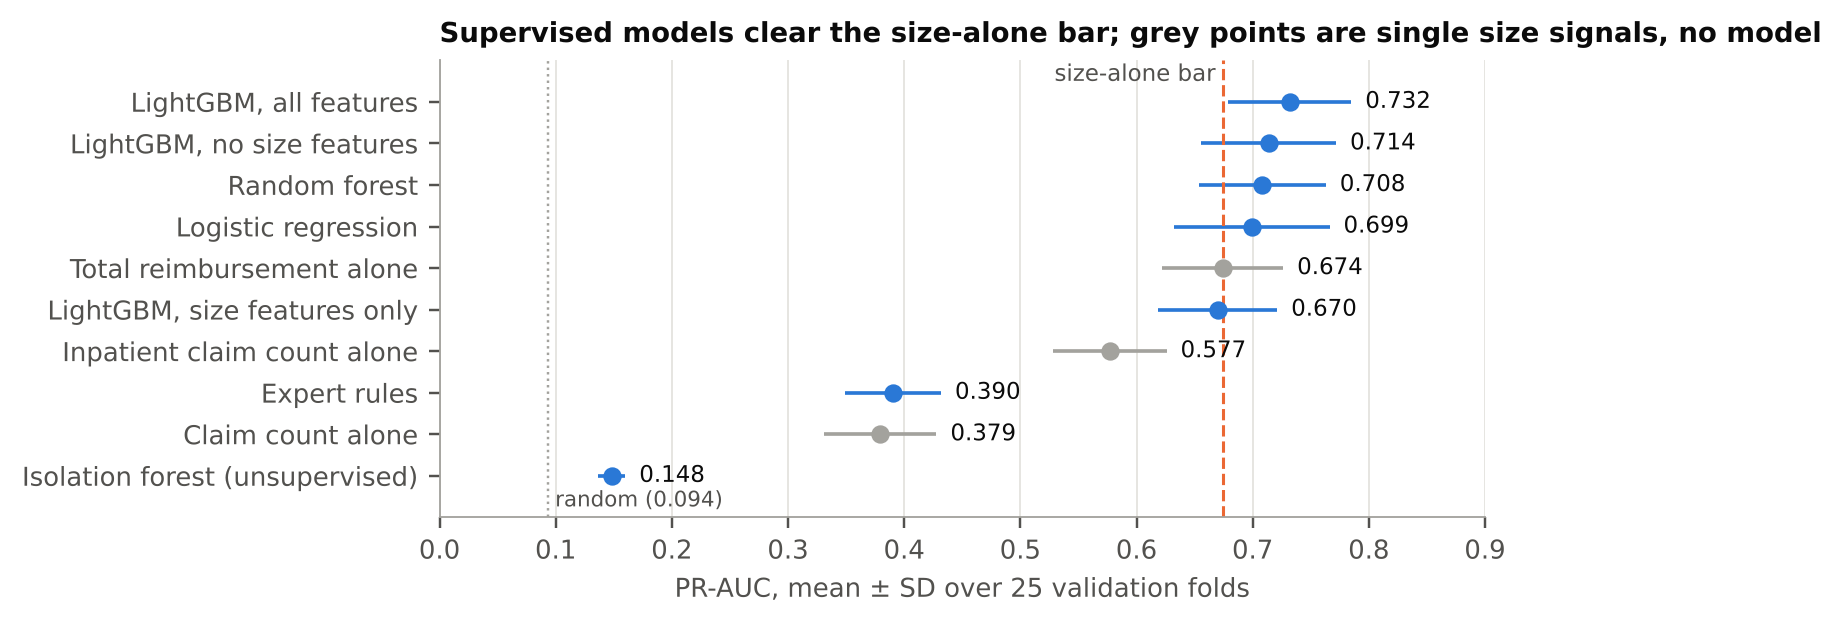
\includegraphics[width=\linewidth]{fig2_models_cv.png}
\caption{Cross-validated PR-AUC. A random ranking scores 0.094. Total reimbursement alone (dashed) is the bar.}\label{fig:models}
\end{figure}

Total reimbursement alone reaches PR-AUC $0.674\pm0.052$ (ROC-AUC 0.934). Its ROC-AUC is within 0.02 of the 0.95 reported by a published stacking ensemble on this dataset \cite{hasan2025}, which suggests that headline scores on this benchmark mostly measure size. Claim count alone does far worse (0.379) because a provider with many cheap outpatient visits is rarely flagged: money and inpatient care matter more than visits.

LightGBM is the best model at $0.732\pm0.053$, ahead of size alone on all 25 folds (mean paired gain $+0.058\pm0.026$), of the random forest on 23 (+0.024) and of logistic regression on 22 (+0.032). The gain over size is real but modest: the model's lead is concentrated in the top of the queue, where audits happen (Fig.~\ref{fig:test}). Expert rules (0.390) do worse than size alone because rules fire independently and a provider tripping many weak rules outranks one that is extreme on the strong one. Isolation Forest (0.148) barely beats random: the providers it finds anomalous are not the flagged ones, so ``unusual'' and ``flagged'' are different concepts here.

\subsection{E2: what matters beyond size}

A LightGBM given no size features still reaches $0.714\pm0.058$, better than size alone on 23 of 25 folds and better than a LightGBM given only the size features ($0.670$). Behaviour therefore carries signal that size does not. Removing one family at a time from this size-free model (Fig.~\ref{fig:ablation}) shows where it lives: dropping \emph{intensity} costs 0.087, dropping \emph{coding} 0.017, and every other family under 0.01. The families overlap, so ablation measures unique contribution; patient mix and physician concentration slightly \emph{improve} the model when removed, a sign they mostly add noise.

\begin{figure}[H]\centering
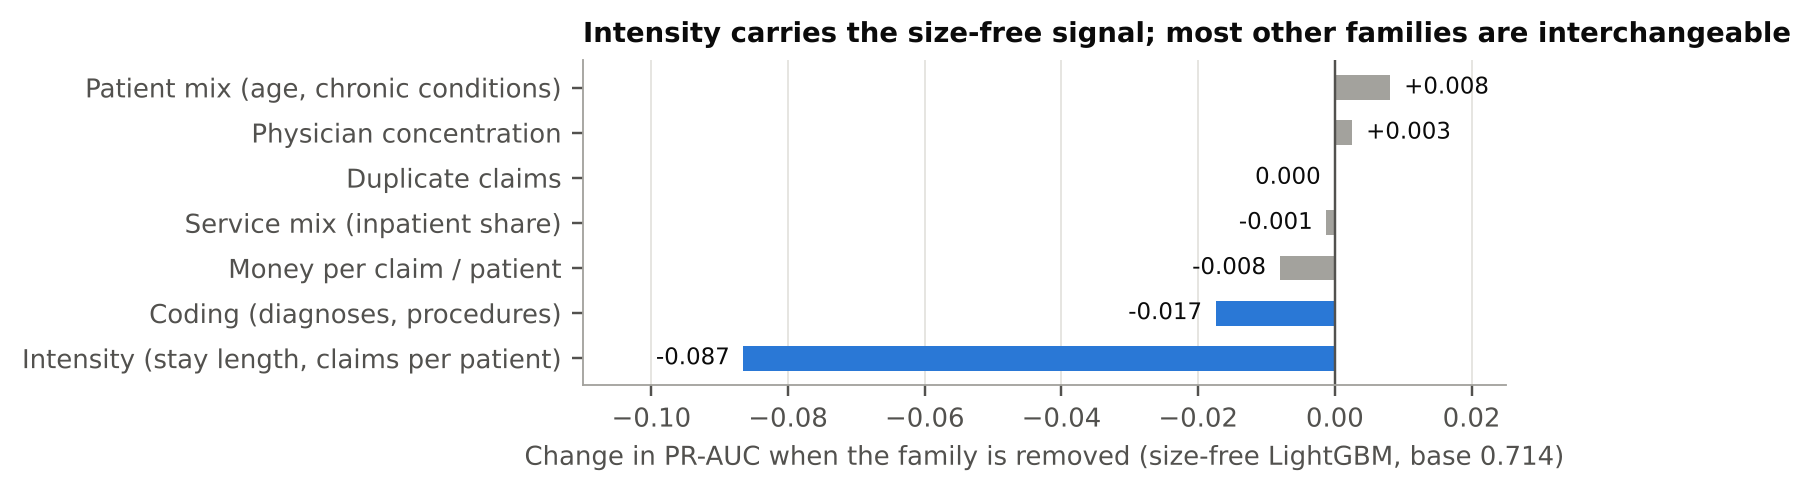
\includegraphics[width=\linewidth]{fig3_ablation.png}
\caption{Change in PR-AUC when one family is removed from the size-free LightGBM (25 folds).}\label{fig:ablation}
\end{figure}

SHAP values on the test set (Fig.~\ref{fig:shap}) agree. With all features, total reimbursement is the largest driver, followed by maximum length of stay and claims per beneficiary. Without size features the model leans on the same intensity measures plus distinct primary diagnoses per claim and the maximum inpatient payment. In investigator terms the size-free model flags providers whose patients stay unusually long, who bill each patient repeatedly, and whose diagnosis coding varies widely: patterns the playbook links to excessive stays (T7), phantom billing (T1) and misrepresented services (T3).

\begin{figure}[H]\centering
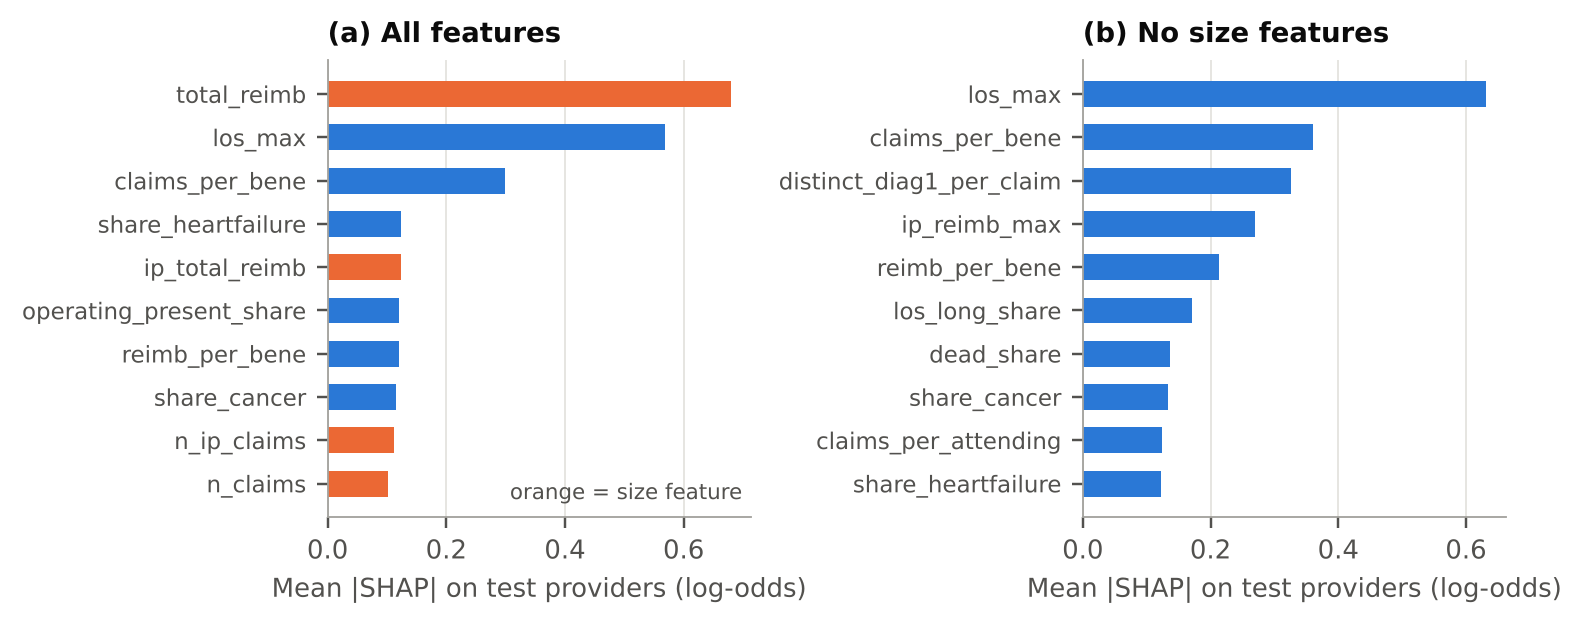
\includegraphics[width=\linewidth]{fig5_shap.png}
\caption{Mean absolute SHAP value on the 1,082 test providers, top 10 features. Orange marks size features.}\label{fig:shap}
\end{figure}

\subsection{E3, E5, E7: network, imbalance and label noise}

\textbf{Network (E3).} The lecture 08 homophily test, comparing the observed share of cross-label links with the expected $2lf$, gives 0.367 against 0.170, which would suggest flagged providers avoid each other. But flagged providers are large and hold many links: 23.8\% of link ends sit on flagged providers although they are 9.4\% of providers. Against a degree-preserving expectation of 0.362, the observed 0.367 shows no homophily ($z=3.4$ in the heterophilic direction). Consistently, network features change PR-AUC by +0.001 (13 of 25 folds better) and by +0.002 on the test set (95\% CI $-0.011$ to $+0.016$). We report this as a negative result and a methodological lesson: the naive homophily test confounds degree with label. It also fits the synthetic-data hypothesis, since DE-SynPUF assigns provider codes at random.

\textbf{Imbalance (E5).} For ranking, class weights barely matter (LightGBM $0.732$ with, $0.731$ without) and SMOTE slightly hurts ($0.717$); for logistic regression SMOTE costs 0.027 against no reweighting. Ranking metrics are threshold-free, so reweighting mostly shifts scores without reordering providers, while synthetic minority points interpolate between heterogeneous flagged providers. Weighting does distort calibration: the logistic model's Brier score doubles from 0.045 to 0.090 with class weights. If calibrated probabilities are needed for expected-loss ranking, the unweighted model should be used.

\textbf{Label noise (E7).} If some flagged providers were never caught, training labels contain hidden positives. Relabelling 10\%, 20\%, 30\% and 50\% of training positives as negatives lowers PR-AUC on clean validation labels from 0.732 to 0.718, 0.707, 0.686 and 0.664 (Fig.~\ref{fig:noise}). The model degrades gracefully, staying above the size-alone bar at 30\% missing flags (0.686 vs 0.674) and falling below it by 50\%, which bounds how much behavioural signal survives imperfect labels.

\begin{figure}[H]\centering
\begin{minipage}[t]{0.42\linewidth}\vspace{0pt}
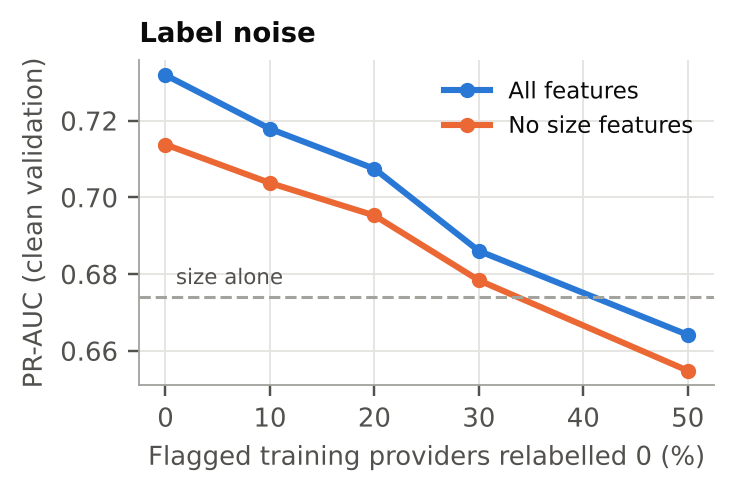
\includegraphics[width=\linewidth]{fig6_noise.png}
\end{minipage}\hfill
\begin{minipage}[t]{0.55\linewidth}\vspace{0pt}
\small
\captionof{table}{E9: claim-level LightGBM, random claim split vs provider-grouped split. Claim PR-AUC should be read against the claim base rate.}\label{tab:e9}
\begin{tabular}{@{}llcc@{}}
\toprule
Features & Split & Base & PR-AUC \\
\midrule
Claim only & random & 0.380 & 0.435 \\
 & grouped & 0.446 & 0.484 \\
+ IDs & random & 0.380 & \textbf{0.868} \\
 & grouped & 0.446 & 0.542 \\
\bottomrule
\end{tabular}
\end{minipage}
\caption{Left: PR-AUC under hidden positives in training (25 folds); dashed: size alone.}\label{fig:noise}
\end{figure}

\subsection{E9: how much a leaky split inflates results}\label{sec:e9}

A common design in public analyses of this dataset is to model claims, attach the provider's label to each claim, and split the claims at random. We reproduced that design with a claim-level LightGBM, with and without integer-encoded physician, state and county identifiers (Table~\ref{tab:e9}). With identifiers and a random split, claim-level PR-AUC is 0.868 (base rate 0.380); with a provider-grouped split it is 0.542 (base 0.446). The mechanism is concrete: 93.6\% of the 82,063 attending physicians bill for a single provider, so a physician ID identifies the provider, and under a random split 91.9\% of test claims have a physician already seen in training, against 9.8\% under the grouped split. The model memorises providers, not behaviour. Without identifiers the claim model is barely above its base rate under either split, confirming that the signal is a provider-level pattern. The two published studies we found report their split only as ``80/20'' or not at all \cite{hasan2025,ahammed2026}.

\subsection{Held-out test set and operating point (E6)}

\begin{table}[H]\centering\small
\caption{Held-out test set (1,082 providers, 101 flagged), scored once. Brackets: bootstrap 95\% CI.}\label{tab:test}
\begin{tabular}{lcccccc}
\toprule
Model & PR-AUC & ROC-AUC & P@50 & P@100 & R@100 & P@54 (5\%) \\
\midrule
Total reimbursement alone & 0.743 [0.670, 0.815] & 0.954 & 0.84 & 0.69 & 0.68 & 0.85 \\
Expert rules & 0.404 [0.340, 0.492] & 0.905 & 0.46 & 0.45 & 0.45 & 0.43 \\
Isolation Forest & 0.158 [0.142, 0.186] & 0.739 & 0.04 & 0.08 & 0.08 & 0.04 \\
Logistic regression & 0.775 [0.705, 0.848] & 0.969 & 0.88 & 0.69 & 0.68 & 0.89 \\
Random forest & 0.782 [0.713, 0.853] & 0.972 & 0.82 & 0.72 & 0.71 & 0.83 \\
\textbf{LightGBM} & \textbf{0.805 [0.740, 0.867]} & 0.972 & 0.86 & \textbf{0.74} & \textbf{0.73} & 0.87 \\
LightGBM, no size features & 0.784 [0.716, 0.853] & 0.969 & 0.86 & 0.71 & 0.70 & 0.87 \\
LightGBM + network & 0.807 [0.742, 0.867] & 0.972 & 0.88 & 0.72 & 0.71 & 0.87 \\
\bottomrule
\end{tabular}
\end{table}

The test ranking matches cross-validation (Table~\ref{tab:test}); test PR-AUCs are higher for every model, within the fold-to-fold spread. LightGBM beats size alone by 0.062 in PR-AUC (paired bootstrap 95\% CI $+0.023$ to $+0.103$), the only test difference whose interval excludes zero. At $k=100$ it finds 74 flagged providers against 69 for size alone (CI for the gain $-0.02$ to $+0.12$): with 101 positives, the test set is too small to separate close models at a single queue size, which is why the repeated folds carry the model choice.

\begin{figure}[H]\centering
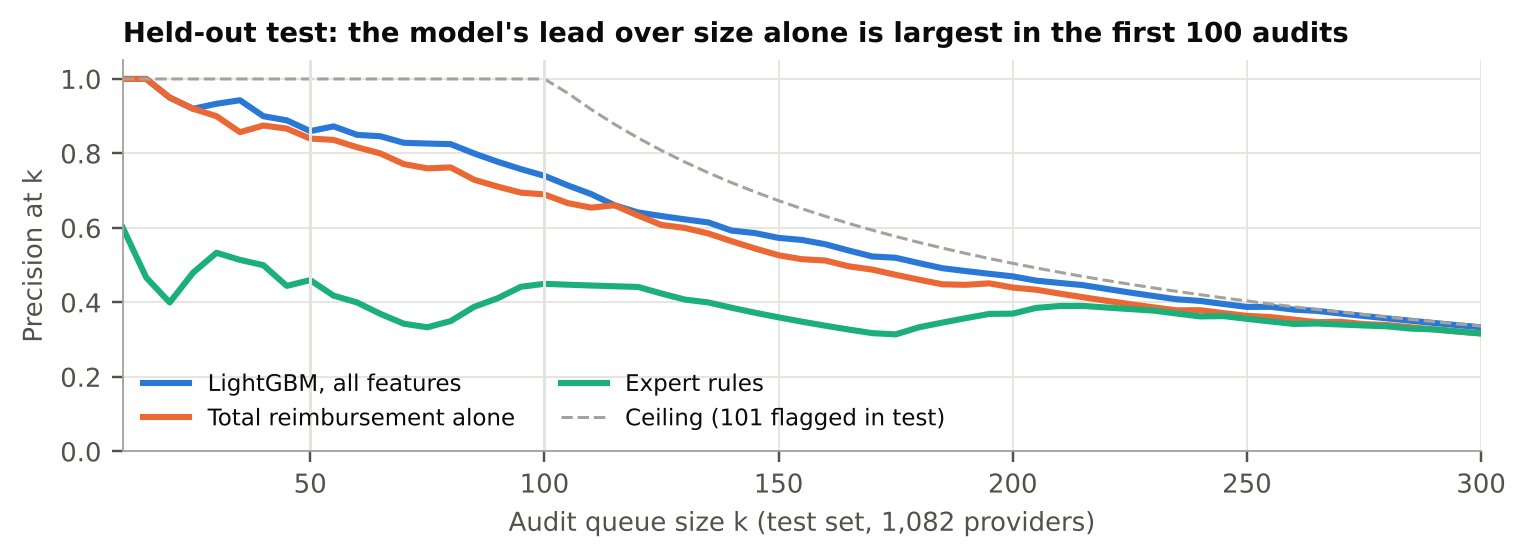
\includegraphics[width=\linewidth]{fig4_test_precision_at_k.png}
\caption{Precision at queue size $k$ on the test set. The dashed ceiling is the best achievable precision with 101 flagged providers.}\label{fig:test}
\end{figure}

\textbf{Choosing the queue size.} The right $k$ depends on the cost of missing a flagged provider (FN) relative to a wasted audit (FP). For each cost ratio we chose the queue share that minimised FP $+$ ratio$\times$FN on the development set's out-of-fold scores, then applied it to the test set (Table~\ref{tab:ops}). At 5:1 the queue holds 17\% of providers and catches 90\% of flagged ones at 49\% precision; even at 50:1 the model's cost (264) is a quarter of auditing everyone (981).

\begin{table}[H]\centering\small
\caption{E6: operating points on the test set; queue share chosen on development folds.}\label{tab:ops}
\begin{tabular}{rrrrrrrrr}
\toprule
FN:FP cost & Queue & TP & FP & FN & Precision & Recall & Cost & Cost, audit all \\
\midrule
5:1 & 184 & 91 & 93 & 10 & 0.49 & 0.90 & 143 & 981 \\
10:1 & 206 & 94 & 112 & 7 & 0.46 & 0.93 & 182 & 981 \\
20:1 & 238 & 97 & 141 & 4 & 0.41 & 0.96 & 221 & 981 \\
50:1 & 314 & 100 & 214 & 1 & 0.32 & 0.99 & 264 & 981 \\
\bottomrule
\end{tabular}
\end{table}

\subsection{Agent experiments (E4, E8, E10)}

\textbf{Retrieval quality (no LLM needed).} On 20 gold queries written with different vocabulary from the playbook (two per section), hybrid retrieval reaches recall@1 0.90, recall@3 1.00 and MRR 0.933, against 0.85 / 1.00 / 0.925 for BM25 alone and 0.80 / 0.85 / 0.857 for the dense index alone. As lecture 06 argues, fusion beats either ranker; with only ten sections, the absolute values are optimistic.

\textbf{Run.} All agents ran on Claude Sonnet 5.5 at low effort: 60 calls, 141,625 input and 47,505 output tokens, US\$0.76 in total, with every response passing schema validation at the first attempt. The run was made on one machine (Windows) and replayed from its cache on another (Linux) with identical results.

\begin{table}[H]\centering\small
\caption{E4: agent-assisted vs fixed pipeline on the same 25 folds. Configurations were chosen by the agents on the first CV repeat.}\label{tab:e4}
\begin{tabular}{llccc}
\toprule
Pipeline & Configuration chosen & PR-AUC & vs fixed & Folds better \\
\midrule
Fixed (E1) & LightGBM, all, class weights & $0.732\pm0.053$ & -- & -- \\
Agents, run 1 & Random forest, all & $0.735\pm0.054$ & $+0.003$ & 17/25 \\
Agents, run 2 & Random forest, all, class weights & $0.705\pm0.056$ & $-0.027$ & 2/25 \\
Agents, run 3 & Logistic, all + agent features & $0.707\pm0.057$ & $-0.025$ & 5/25 \\
No Critic (run 1) & LightGBM, all + agent features & $0.728\pm0.054$ & $-0.004$ & 10/25 \\
No Feature agent & Logistic, all, class weights & $0.694\pm0.065$ & $-0.038$ & 2/25 \\
\bottomrule
\end{tabular}
\end{table}

\textbf{E4: the agents did not beat the fixed pipeline.} Across three runs the agent pipeline averaged 0.716 against 0.732, and its result swung from 0.705 to 0.735 depending on the run (Table~\ref{tab:e4}). The logs show why. In every run the Experiment agent's own best configuration was a LightGBM with agent features (0.736--0.739 on the tuning folds), but the Critic, following our prompt's rule to prefer a simpler model unless a complex one wins by more than one standard deviation across folds, chose a random forest or logistic regression. That rule is statistically wrong: the fold SD ($\approx0.06$) measures how much one model's score moves between folds, whereas two models scored on the same folds differ far more consistently (LightGBM beats the random forest on 23 of 25 folds, paired SD 0.016). Without the Critic, the agents' best first-round configuration is within noise of the fixed pipeline ($-0.004$). The Feature agent's 20 proposed features (19--20 passed the Leakage agent) added nothing beyond ours. The lesson is about design, not capability: an LLM critic applies the statistical rule it is given faithfully, so the rule must compare models on paired folds. Asked to flag results that look too good, the Critic independently suggested the label may be derived from the same billing features, the conclusion E0 reached.

\textbf{E10: the Leakage agent caught every planted leak.} Across three reviews of 15 feature specifications it flagged all 5 leaks each time (15/15) with no false alarms. Twice it marked the network degree feature ``uncertain'' because the graph includes test providers' claims; that is a fair point, and our design accepts it because claims are known for every provider at scoring time. The Cleaning agent's 42-step plan matched 6 of our 7 checklist items and never imputed structurally missing fields; the difference was keeping the constant inpatient deductible as a missing-value indicator rather than dropping it, the kind of choice the human approval gate exists to settle.

\textbf{E8: case briefs were faithful, and retrieval changed the decision.} The agent wrote briefs for the 20 highest-ranked test providers, 19 of them flagged. All 198 drivers were copied exactly (value, peer percentile and SHAP), all 44 citations named a section that had been retrieved for that provider and that lists one of the brief's drivers, and none of the 40 briefs stated fraud as fact: every one called the label a suspicion. Without the playbook the agent cited nothing, as instructed. The playbook changed the recommendation: without it all 20 providers went to priority audit; with it, 11 of 20 were downgraded to desk review, citing the section that says volume alone is not evidence of fraud (T6 was cited in 20 briefs, excessive stays T7 in 19). Retrieval thus carried our central finding, size versus behaviour, into the investigator's queue, at 1.3 US cents per brief against 0.9 without it. The checks are deterministic proxies: they verify that numbers and citations are right, not that an investigator finds the brief useful. (Our first version of the confirmed-fraud check counted hedges such as ``not confirmed fraud'' as claims; the corrected check handles negation and found none.)

\subsection{Integration into an audit workflow}

The model's output is a ranked queue, not a verdict. A practical cycle (lecture 01's detect--investigate--confirm--prevent loop):
\begin{enumerate}
\item \textbf{Score monthly.} Re-aggregate each provider's last 12 months of claims and score every provider; scoring 5,000 providers takes seconds.
\item \textbf{Size the queue by capacity and cost.} Use Table~\ref{tab:ops}: e.g.\ an 80-audit capacity takes the top 80; a team that rates a missed case at 10 audits takes about 19\% of providers.
\item \textbf{Brief before auditing.} The Case-file agent attaches the drivers, peer percentiles and cited playbook sections. Investigators see \emph{why} a provider ranks high, in particular whether it is size alone (a large hospital) or intensity and coding (a behavioural pattern), which deserve different responses: a desk review versus a field audit. In E8 the grounded agent made exactly this split, sending 11 of the top 20 to desk review.
\item \textbf{Human decision, then feedback.} No payment is denied by the model. Confirmed and cleared outcomes return as new labels, replacing the undocumented ones, and the model is retrained.
\end{enumerate}
Two operational risks follow from our results. A size-driven model will repeatedly send the same large hospitals to audit; the size-free score should be shown beside the main score so that reviewers can tell behaviour from bulk. Patient-mix features can penalise providers who treat sicker patients; E2 shows they can be dropped at no cost, and we recommend doing so in deployment.

%=====================================================================
\section{Conclusion}

\textbf{Findings.} (1) On this benchmark the label is largely a size signal: total reimbursement alone gives PR-AUC 0.674 and ROC-AUC 0.934. (2) LightGBM adds a consistent margin (0.732, all 25 folds better; 0.805 vs 0.743 on test, CI excluding zero), and a size-free model keeps most of it (0.714), carried by care intensity and coding breadth. (3) Network links, resampling, expert rules and anomaly detection add nothing; the apparent network heterophily disappears once degree is accounted for. (4) A claim-level random split inflates PR-AUC from 0.542 to 0.868 by memorising physician IDs, a likely source of optimistic published results. (5) The agents add value as reviewers and briefers, not as modellers: build-time agents lost 0.016 on average to a fixed pipeline because of an unpaired decision rule, while the Leakage agent was perfect on planted leaks and grounded briefs were faithful, cheap and sensitive to the size-versus-behaviour distinction.

\textbf{Limitations.} \emph{Data:} the claims appear to be synthetic and the label's origin is unknown, so results describe this benchmark, not real Medicare providers; 13 months of single-label data cannot show drift or how fraudsters adapt to a deployed model (lecture 07's evasion risk). \emph{Evaluation:} the test set has only 101 positives, so close models are not separable at one queue size; tuning and evaluation share the development data (tuning used the first CV repeat), a small optimistic bias applied equally to all tuned models. \emph{Agents:} LLM outputs are not deterministic (sampling cannot be fixed on current models), and three runs gave PR-AUC from 0.705 to 0.735; the Critic's rule came from our prompt, so E4 tests our design as much as the model; the leak benchmark and checklist are small and written by us, as is the ten-section retrieval corpus; brief usefulness was not tested with investigators. \emph{Fairness:} size and patient-mix features can disadvantage large or high-acuity providers.

\textbf{Future directions.} Give the Critic paired fold differences and re-run E4; replace the label with audit outcomes and evaluate on a later period; add claim-line codes (HCPCS) to observe unbundling and non-covered billing, which this data cannot show; test the size-free score with investigators to see whether it changes which audits they open; and run the agent layer with an open-weights model inside the payer's network, since claims contain protected health data (lecture 05).

%=====================================================================
\begin{thebibliography}{99}\small\setlength{\itemsep}{1pt}
\bibitem{kaggle} R. A. Gupta. \emph{Healthcare Provider Fraud Detection Analysis} [dataset]. Kaggle. \url{https://www.kaggle.com/datasets/rohitrox/healthcare-provider-fraud-detection-analysis}
\bibitem{synpuf} Centers for Medicare \& Medicaid Services. \emph{CMS 2008--2010 Data Entrepreneurs' Synthetic Public Use File (DE-SynPUF)}. \url{https://www.cms.gov/data-research/statistics-trends-and-reports/medicare-claims-synthetic-public-use-files/cms-2008-2010-data-entrepreneurs-synthetic-public-use-file-de-synpuf}
\bibitem{synpufdug} Centers for Medicare \& Medicaid Services. \emph{DE-SynPUF Data Users Guide}. \url{https://www.cms.gov/Research-Statistics-Data-and-Systems/Downloadable-Public-Use-Files/SynPUFs/Downloads/SynPUF_DUG.pdf}
\bibitem{hasan2025} A. M. Hasan, R. Al-Yakzan, B. Alkhatib. Developing and using data mining to detect healthcare fraud and abuse for health insurance companies. \emph{Research Square} preprint, 2025. \url{https://www.researchsquare.com/article/rs-7558249/v1}
\bibitem{ahammed2026} F. Ahammed, B. Al Barakati, O. Marques. Improving Medicare fraud detection accuracy in deep learning by exploring feature selection and data sampling techniques. \emph{medRxiv} preprint, 2026. doi:10.64898/2026.03.18.26348763
\bibitem{lightgbm} G. Ke et al. LightGBM: A highly efficient gradient boosting decision tree. \emph{NeurIPS}, 2017.
\bibitem{treeshap} S. M. Lundberg et al. From local explanations to global understanding with explainable AI for trees. \emph{Nature Machine Intelligence} 2:56--67, 2020.
\bibitem{smote} N. V. Chawla, K. W. Bowyer, L. O. Hall, W. P. Kegelmeyer. SMOTE: Synthetic minority over-sampling technique. \emph{JAIR} 16:321--357, 2002.
\bibitem{rrf} G. V. Cormack, C. L. A. Clarke, S. B\"uttcher. Reciprocal rank fusion outperforms Condorcet and individual rank learning methods. \emph{SIGIR}, 2009.
\bibitem{saito} T. Saito, M. Rehmsmeier. The precision-recall plot is more informative than the ROC plot when evaluating binary classifiers on imbalanced datasets. \emph{PLOS ONE} 10(3):e0118432, 2015.
\bibitem{baesens} B. Baesens, V. Van Vlasselaer, W. Verbeke. \emph{Fraud Analytics Using Descriptive, Predictive, and Social Network Techniques}. Wiley, 2015.
\bibitem{lectures} BT4012 Fraud Analytics lecture notes 01--08, National University of Singapore, 2026.
\end{thebibliography}

\appendix
\section*{Appendix A. Reproducibility}
\small\sloppy
Every number in this report is written by the scripts to \texttt{results/tables/}: \texttt{data\_quality.json} (Table~\ref{tab:data}), \texttt{cv\_summary.csv} and \texttt{cv\_paired\_diffs.csv} (E0--E3, E5, E7), \texttt{homophily.json}, \texttt{e5\_calibration.csv}, \texttt{test\_results.csv} and \texttt{test\_paired\_diffs.csv} (Table~\ref{tab:test}), \texttt{e6\_operating\_points.csv}, \texttt{e9\_leakage.csv}, \texttt{e9\_physicians.json}, and \texttt{agents/}. The pipeline is \texttt{01\_build\_features.py} $\rightarrow$ \texttt{02\_run\_experiments.py} $\rightarrow$ \texttt{03\_run\_agents.py} $\rightarrow$ \texttt{04\_make\_figures.py}; seeds are fixed in \texttt{config.py}; the README lists versions and run times (about 20 minutes on two cores). The raw data is not redistributed; the README explains how to obtain it.

\section*{Appendix B. Response to proposal feedback}
\begin{tabularx}{\linewidth}{p{5.2cm}X}
\toprule
Feedback & Where addressed \\
\midrule
Origin and meaning of PotentialFraud & \S2: undocumented; data matches synthetic DE-SynPUF; treated as suspicion; E7 tests hidden positives \\
Time range; fraud and non-fraud counts & Table~\ref{tab:data} \\
Kaggle test files unlabelled; $k$ vs test size & Evaluation on labelled providers only; $k\in\{50,100,5\%,10\%\}$ with ceilings (Fig.~\ref{fig:test}) \\
At least three baselines & Size alone, expert rules, logistic regression, random forest, LightGBM, Isolation Forest (E0--E1) \\
Agent pipeline vs fixed pipeline, same split & E4 on identical folds, three runs, Critic and Feature agent ablations (Table~\ref{tab:e4}) \\
Precision@$k$, recall@$k$, PR-AUC; stability & All three reported; 25 repeated folds (mean $\pm$ SD, paired gains); bootstrap CIs on test \\
\bottomrule
\end{tabularx}

\end{document}
